\chapter{Proposed methodology}\label{methodology}

\lettrine{T}{unable} applications are characterized by the presence of specific parameters, also known as \textit{knobs}, that influence program execution; their change produces different application results in terms of metric of interest values, as, for instance, throughput or power consumption. Figure \ref{fig::appDef} shows a typical parallel architecture in witch several tunable applications are running:

\begin{figure}[H]

    \centering
    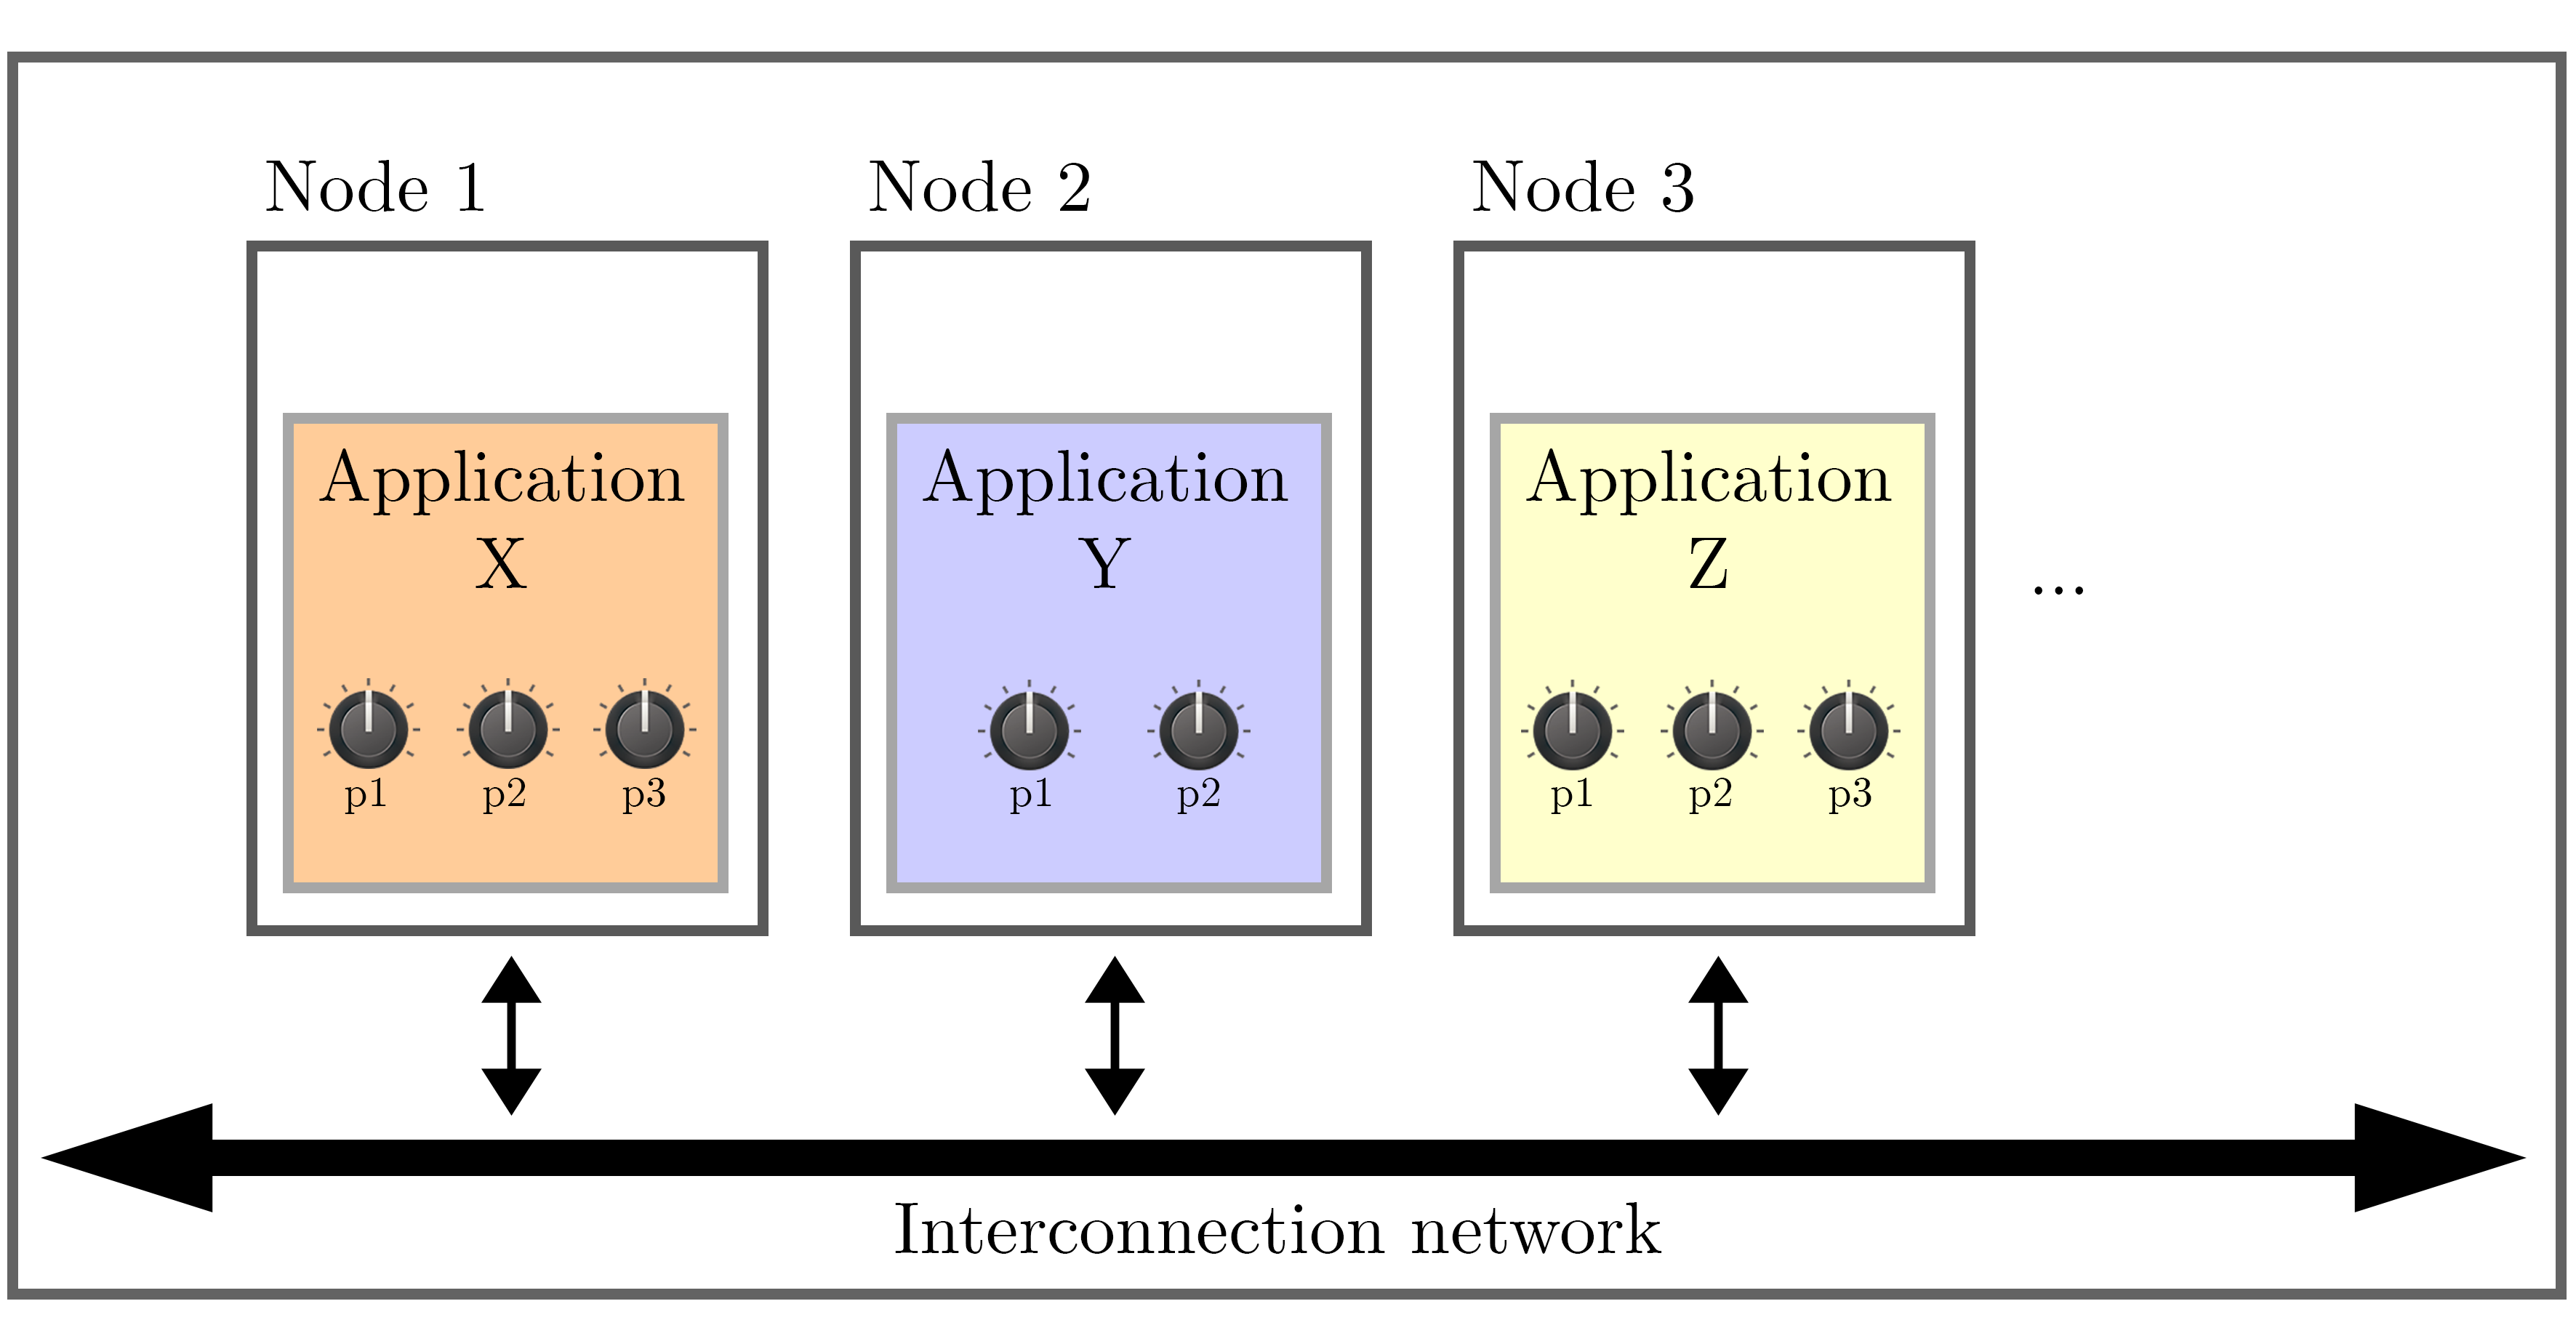
\includegraphics[width = \textwidth]{Apps}
    \caption{An example of a parallel architecture with several executing tunable applications}
    \label{fig::appDef}
    
\end{figure}

Very often, High Performance Computing applications expose a large set of parameters, making related Design Space huge and, consequently, unrealistic to explore it in an exhaustive way; in order to choose, from time to time, best program setting with the aim to improve energy efficiency with respect to power consumption and current input data, the concept of runtime autotuning is used: a class of online autotuners is able to choose, from time to time, best possible parameter values that fullfil application goals and requirements, starting from a design-time knowledge that gives information about parameter values and corresponding metric of interest values, built off-line. Figure \ref{fig::appAut} shows an application interconnected with mARGOt \cite{gadioli2015application}, a dynamic autotuner developed by our research group:

\begin{figure}[H]

    \centering
    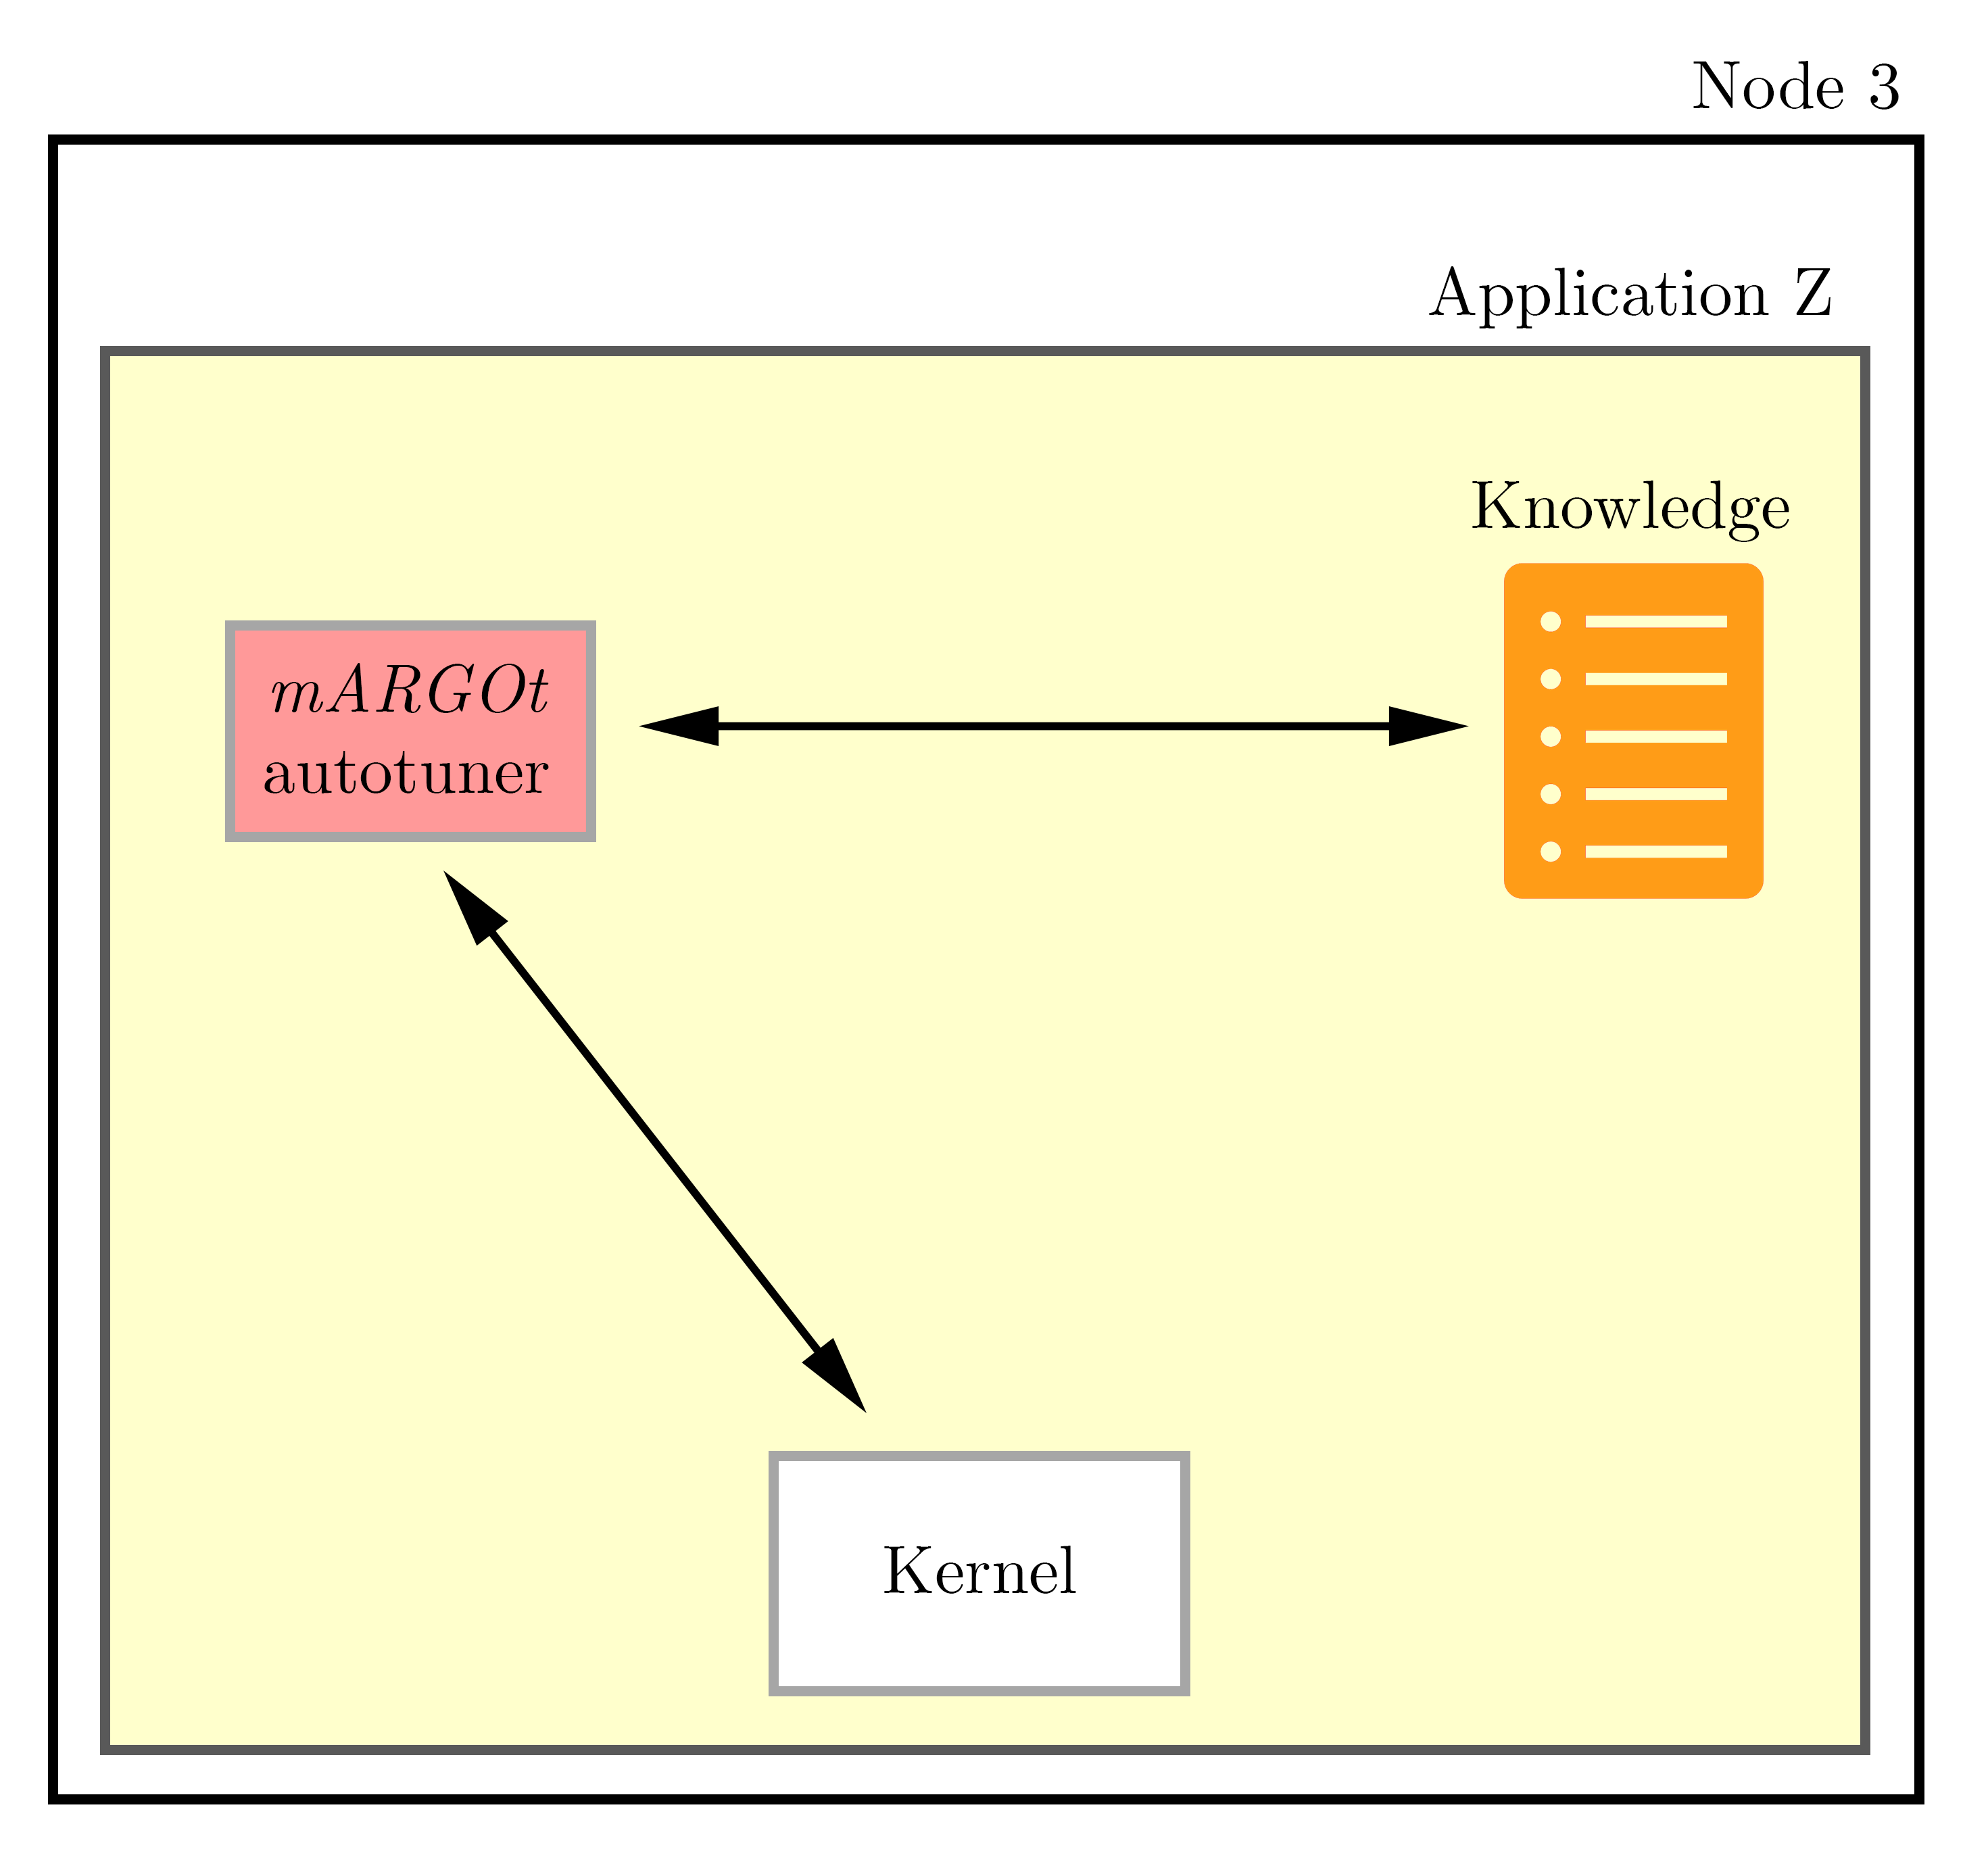
\includegraphics[width = \textwidth]{App_mARGOt}
    \caption{Tunable application with the assistance of mARGOt autotuner schema}
    \label{fig::appAut}
    
\end{figure}

As we can understand, this kind of autotuner needs application knowledge, so there have to be a preceding phase, before program start of computation, in which it is made; our improvement is to avoid this off-line step, building, managing and updating application knowledge during execution itself. A local module mainly takes care of properly setting application knowledge, while a remote one manages collected information during execution, in order to predict complete application model. Figure \ref{fig::appAGORA} shows an application interconnected with Agorà and mARGOt autotuner:

\begin{figure}[H]

    \centering
    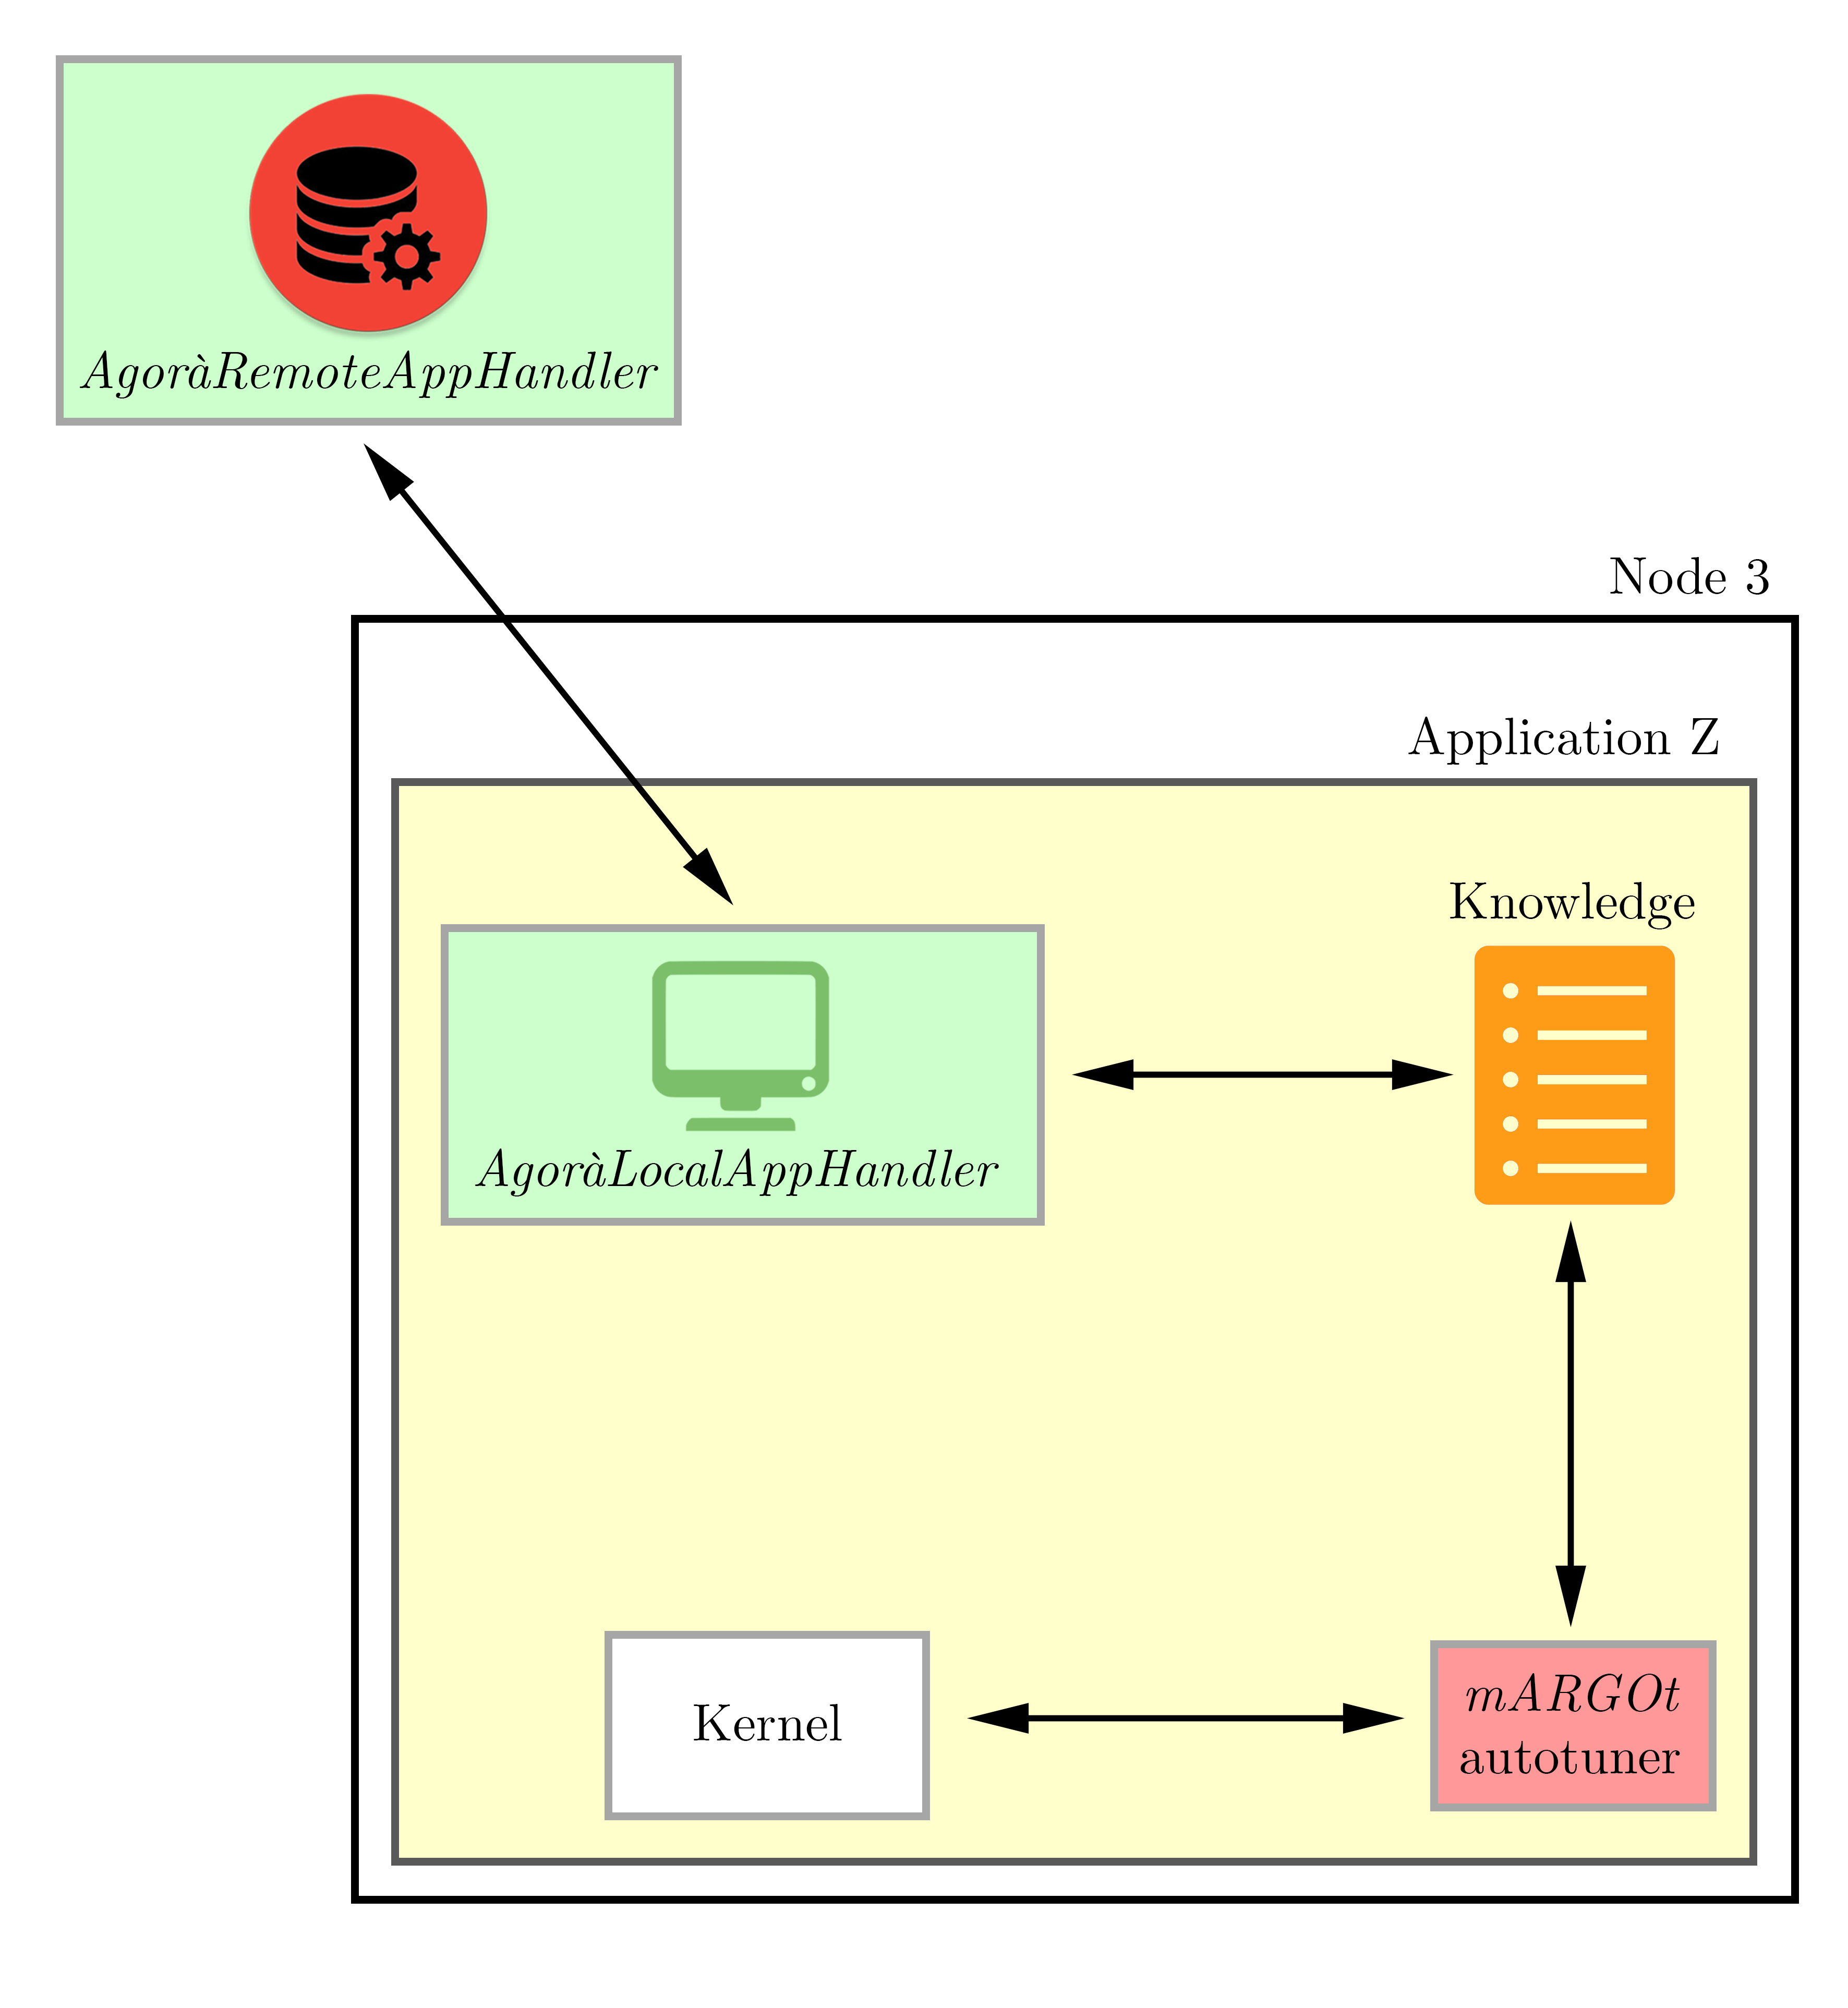
\includegraphics[width = \textwidth]{App_Agora_mARGOt}
    \caption{Tunable application with the assistance of Agorà plus mARGOt autotuner schema}
    \label{fig::appAGORA}
    
\end{figure}

This work, therefore, wants to address the problem of managing possible multiple applications that run, at the same time, inside a parallel architecture; the objective is to initially drive programs execution with a subset of parameters configurations taken from their Design Space, in order to gather all metrics of interest values associated to them; this list will compose the training set for the prediction of the complete model through Machine Learning techniques. Agorà can also correctly manage possible features; a feature is a particular application element than can not be set up like software knobs, but it contributes to the estimation of complete model; during DSE phase, feature values are observed like metric values while, during model prediction, they are considered as parameters, so their observations take part to the estimation of metric of interest values.

The typical architecture in which Agorà works is a parallel one, where there are multiple nodes, potentially heterogeneous, that execute applications; principal Agorà strenghts are:

\begin{enumerate}
    
    \item the ability to drive Design Space Exploration in a distributed way, among all those nodes that are running the same program, in order to considerably reduce DSE phase and to speed up overall workflow;
    
    \item the ability to manage multiple kinds of applications, each of them separately organized by a dedicated Agorà module that is in charge of all the nodes that execute the same program;
    
    \item the out-of-band activity from the parallel architecture data streams: the computation of Design of Experiments configurations, the collection of associated metrics of interest values and the complete models prediction are done in a separate node with respect to the ones that run applications inside the architecture, while the exchange of information is done using the lightweight MQTT protocol (discussed in chapter \ref{mqtt});
    
    \item the persistence of generated knowledge: once the complete model of an application is predicted, it is stored so, at any time, it can be reloaded and it is sent to new nodes that have started running the same application, without repeating all the workflow through which the complete model has been previously predicted;
    
    \item the capability of being fault-tolerant, with respect both to a running node crash and to the interruption of the machine that has the objective to predict applications complete model: if the former situation happens, Agorà has to properly handle the remaining running nodes; if the latter situation happens, running nodes inside the parallel architecture doesn't have to stop their execution but they react properly, according to their internal state at that moment.

\end{enumerate}

\begin{figure}[H]

    \centering
    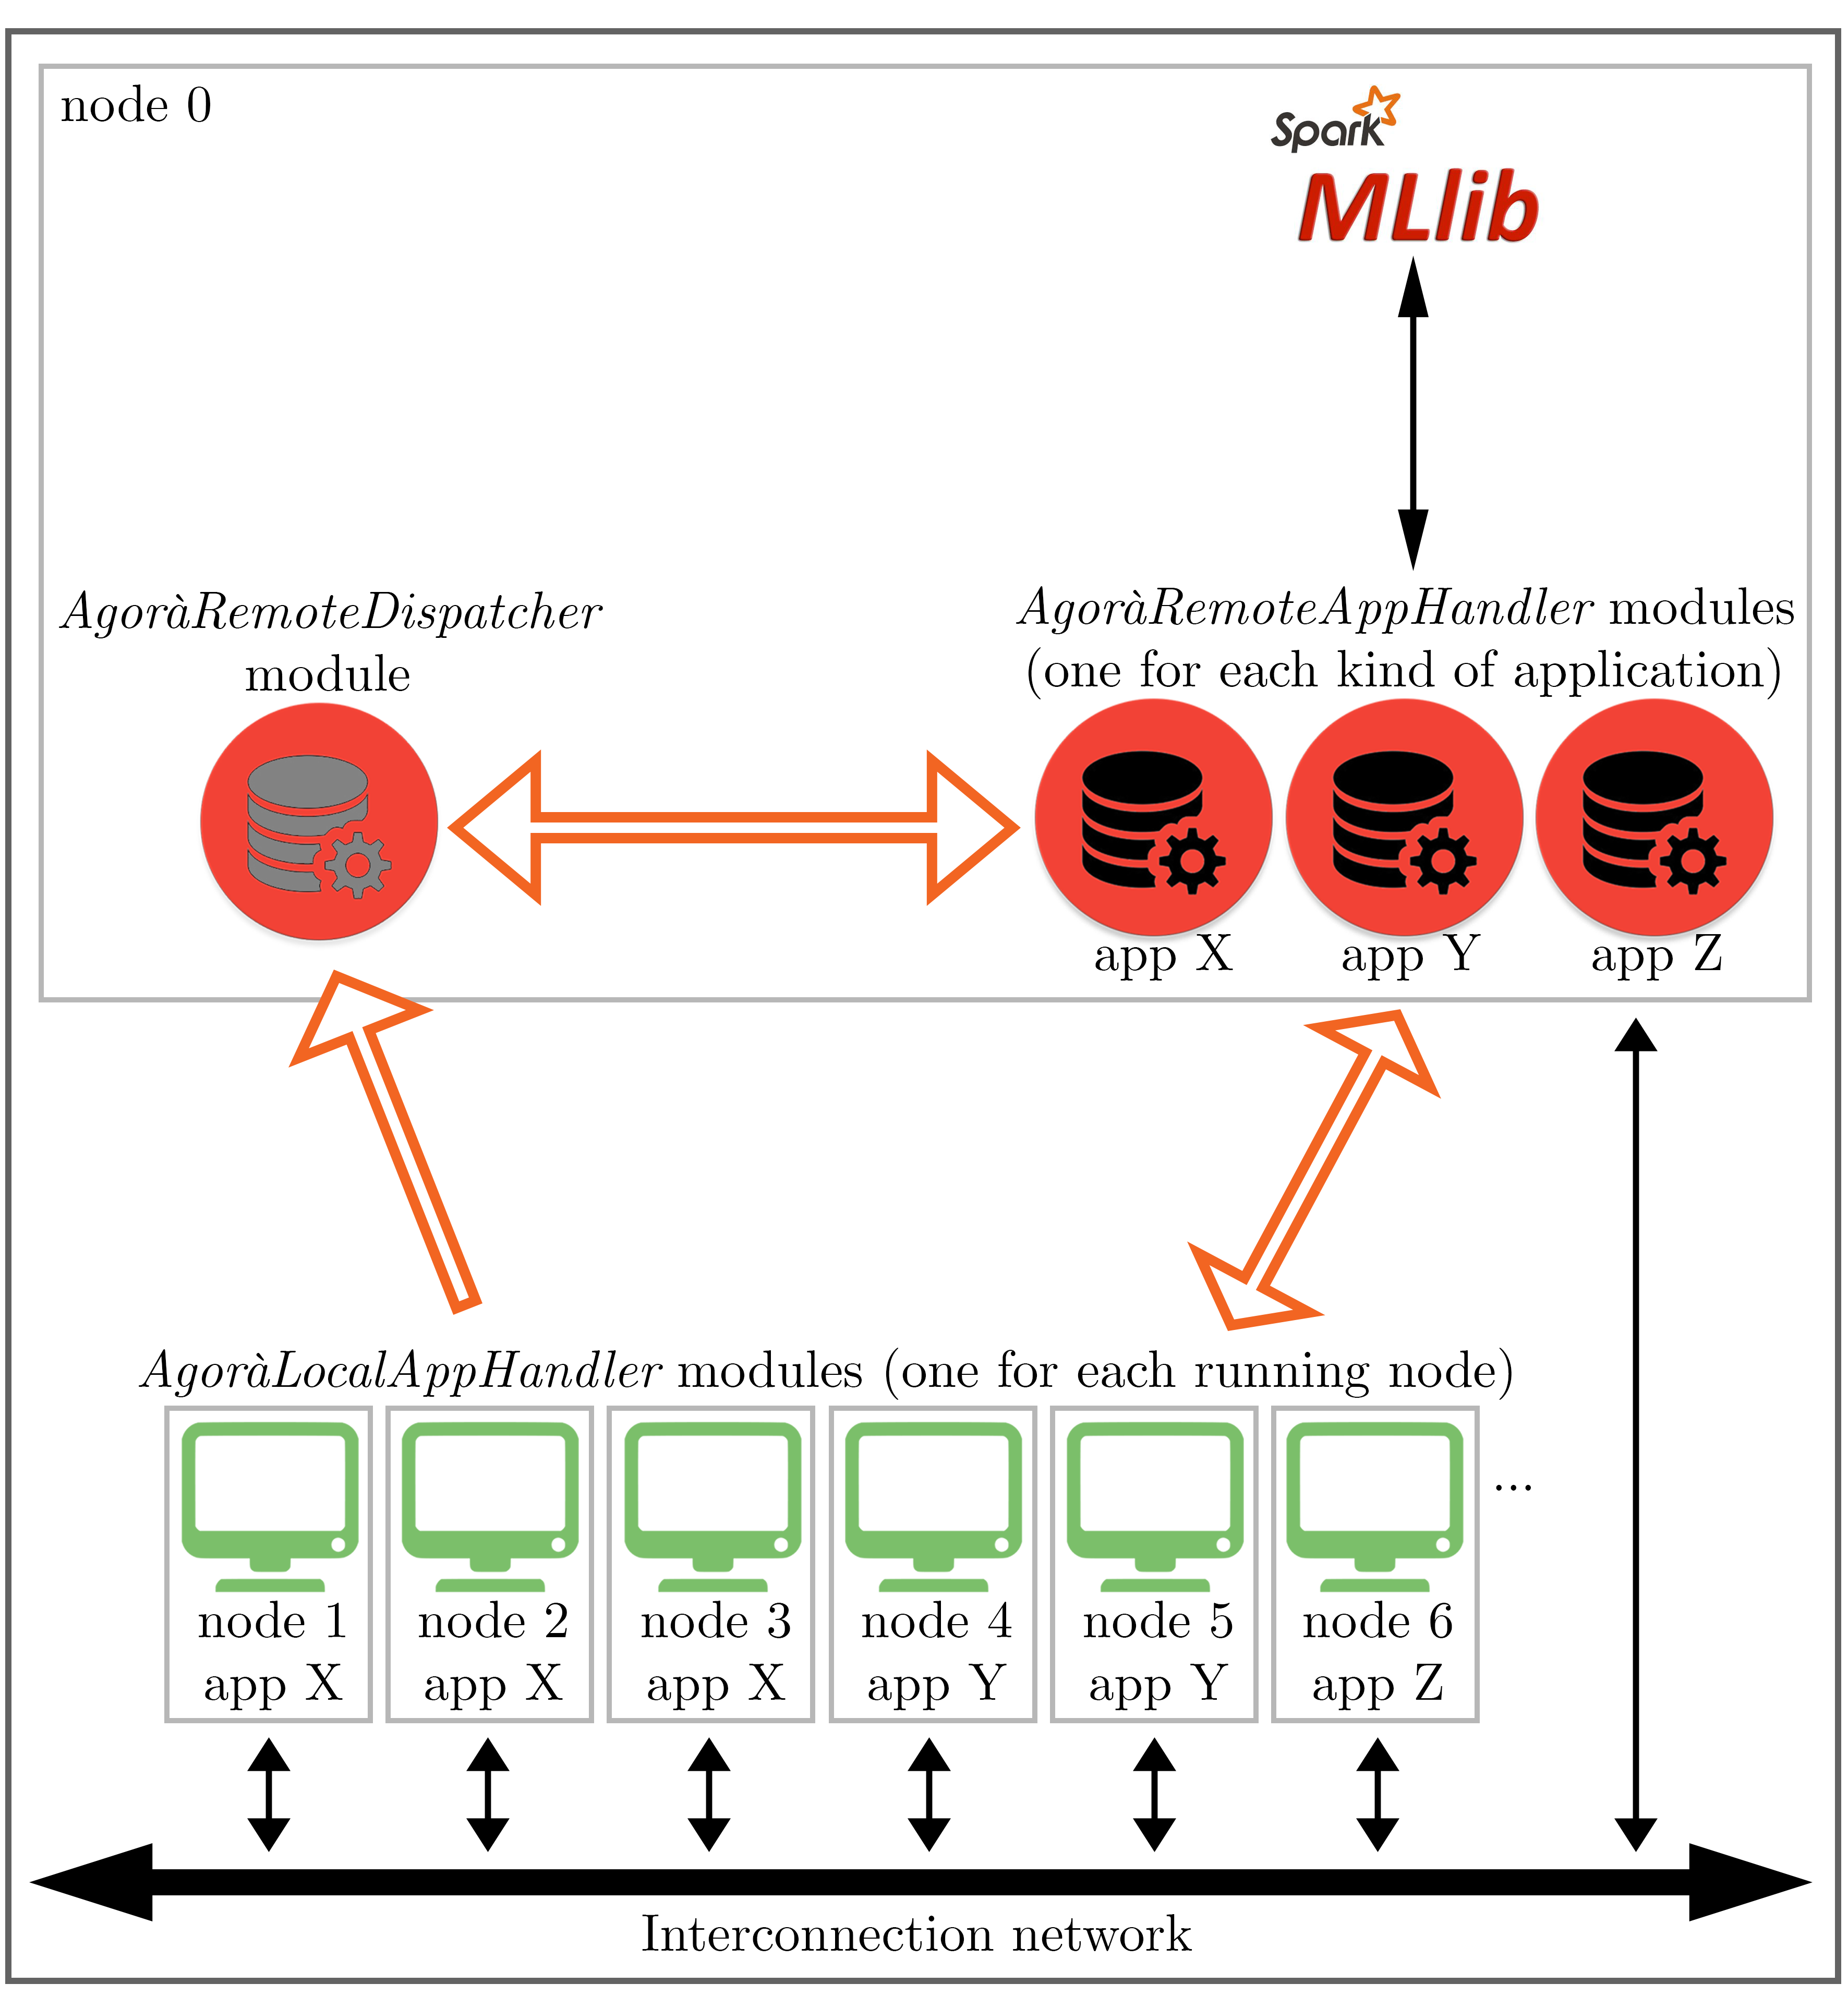
\includegraphics[width = \textwidth]{Agora_overall}
    \caption{Agorà overview in a parallel architecture}
    \label{fig::tesiCris_overview}
    
\end{figure}

Figure \ref{fig::tesiCris_overview} shows all Agorà components and a possible scenario with a parallel architecture in which six nodes are running three different applications; for every kind of application there exists a dedicated AgoràRemoteAppHandler module that manages it; orange arrows represent all possible communications among modules, made possible through MQTT subscriptions and publications on predetermined topics.

Agorà main components are:

\begin{itemize}

    \item the \textit{AgoràDispatcher} module, written in Python: it keeps waiting for programs arrival, in order to properly manage them;
    
    \item the \textit{AgoràRemoteAppHandler} module, written in Python: it is created by the AgoràDispatcher for every kind of application; it asks for application information such as, for instance, all parameters name and values; it computes application configurations that compose the Design of Experiments; it drives Design Space Exploration phase, distributing DoE configurations among all the nodes it manages; it collects parameters values and the observed metrics of interest sent by running programs; it makes use of Machine Learning techniques in order to build the complete application model; it sends the result to connected nodes;
    
    \item the \textit{AgoràLocalAppHandler} module, written in C++: it is set up in every executing program; it communicates with the autotuner that manages application behavior; it notifies the existence of the running machine to the AgoràDispatcher module; it replies to possible information request made by the related AgoràRemoteAppHandler module; during Design Space Exploration phase, it receives configurations from the AgoràRemoteAppHandler module, it pass them to the autotuner and, after the application has done computation, it sends back all the obtained information, regarding parameters values and the associated metrics values; it saves the complete model received from the AgoràRemoteAppHandler module, in order to properly set up the autotuner.

\end{itemize}

Principal use cases that define framework workflow and the interaction among components are the following:

\begin{enumerate}

    \item application start of execution: when programs start running, related AgoràLocalAppHandler module notifies their existence to the AgoràDispatcher module; if the application is unknown, AgoràDispatcher creates a dedicated AgoràRemoteAppHandler module that is in charge of managing it, otherwise it communicates the new node to the corresponding existing AgoràRemoteAppHandler;
    
    \item Design of Experiments computation: AgoràRemoteAppHandler module computes the subset of configurations, from the entire application Design Space, that compose the Design of Experiments; after that, it is ready to drive Design Space Exploration phase, distributing these configurations to requesting nodes;
    
    \item configuration reception: AgoràLocalAppHandler module communicates to the autotuner all the configurations that, from time to time, are sent by the AgoràRemoteAppHandler module; when computation is finished, it sends back to the AgoràRemoteAppHandler module a list of values, made by the configuration just used with the observed metrics of interest;
    
    \item application configurations and related metrics values collection: AgoràRemoteAppHandler module collects all the information it receives from running nodes; when it has all the necessary data, it uses Machine Learning techniques in order to predict the application complete model, made by all possible configurations associated with the predicted metrics values;
    
    \item predicted model dispatch: the complete model is sent by the AgoràRemoteAppHandler to the nodes; AgoràLocalAppHandler set the autotuner with this information, so the application can be set up with the best configuration that fulfills current goals and requirements.

\end{enumerate}

The interaction among Agorà components have been implemented in an asynchronous way: programs executions are independent from the exchange of MQTT messages and all modules properly react to these events, in order to not condition application workflow and to not steal execution time, making all process as flowing as possible.
